\documentclass[ignorenonframetext, hyperref=unicode]{beamer}



\usepackage{cmap}
%\usepackage[T2A]{fontenc}
\usepackage[utf8]{inputenc}
\usepackage[bulgarian]{babel}
\selectlanguage{bulgarian}

\usepackage{color}
\usepackage{graphicx}
\usepackage{listings}
\usepackage{rcsinfo}
\usepackage{pgf}
\usepackage{supertabular}
\usepackage{rotating}

\hypersetup{
	colorlinks=true,
	linkcolor=blue,
	filecolor=blue,
	urlcolor=blue,
	anchorcolor=blue,
	citecolor=blue
}

\lstset{language=C++, 
  numbers=left, 
  numberstyle=\tiny,
  stepnumber=1, 
  numbersep=3pt, 
  tabsize=2, 
  texcl,
  basicstyle=\ttfamily\small,
  identifierstyle=\ttfamily\small,
  keywordstyle=\sffamily\bfseries\small,
  extendedchars=true, inputencoding=utf8,
  backgroundcolor=\color[rgb]{1,1,0.845},
  escapeinside={/*@}{@*/}}

%\usepackage{algpseudocode}
%\usepackage[ruled]{algorithm}

\newcommand{\Cpp}{{\ttfamily\bfseries C++}}
\newcommand{\CC}{{\ttfamily\bfseries C}}

\definecolor{outputcolor}{rgb}{0.0,0.0,0.5}
\newcommand{\aout}[1]{\color{outputcolor}{\begin{verbatim}#1\end{verbatim}}}

% \usepackage[T2A]{fontenc}
% \usepackage[cp1251]{inputenc}
% \usepackage[bulgarian]{babel}
\selectlanguage{bulgarian}




\newcommand{\lubo}{%
\author[Л.~Чорбаджиев]{Любомир Чорбаджиев\inst{1} \\ 
{\ttfamily lchorbadjiev@elsys-bg.org}}
\institute[ELSYS] % (optional, but mostly needed)
{
\inst{1}%
Технологическо училище ``Електронни системи'' \\
Технически университет, София
}}

\newcommand{\osauthors}{%
\author{
	В.Кетипов\\ 
	\and
	Н.Димитров \\ 
	\and
	{Х.Стефанов \\
	{\ttfamily elsys.os.2014@gmail.com}}
}
\institute[ELSYS] % (optional, but mostly needed)
{
\inst{1}%
Технологическо училище ``Електронни системи'' \\
Технически университет, София
}}

\titlegraphic{\href{http://creativecommons.org/licenses/by-sa/3.0/}{
\includegraphics{../macros/cc.png}}}

\newcommand{\ie}{т.~е.\ }

\newcounter{probcounter}[section]
\newenvironment{prob}[1][]%
        {\smallskip%
         \noindent\refstepcounter{probcounter}%
          \textbf{\theprobcounter${}^{#1}$.}\ }%
   {\medskip}

\mode<article>
{

}

\mode<presentation>
{
  \usetheme[secheader=true]{Madrid}
  \usecolortheme{crane}
  \usefonttheme[onlylarge]{structurebold}
  \setbeamercovered{transparent}
}

\usepackage[unicode]{hyperref}

%%% Local Variables: 
%%% mode: latex
%%% TeX-master: t
%%% End: 


\title{Нишки}
\lubo
\date{\today}

\begin{document}

\frame{\maketitle}

\begin{frame}
\frametitle{Съдържание}
\tableofcontents %[hideallsubsections]
\end{frame}

%-------------------------------------------------------------------- SECTION -
\section{Въведение}


%---------------------------------------------------------------------- SLIDE -
\begin{frame}\frametitle{Процеси}
\begin{itemize}
\item Когато операционната система разпределя ресурсите, тя ги разпределя между
процесите, които се изпълняват върху компютърната система. Собствеността на
ресурсите се държи от процесите.
\item Планирането на процесора се извършва в термините на задачи или олекотени
процеси.
\item Операционната система третира тези два аспекта независимо.
\end{itemize}
\end{frame}

%---------------------------------------------------------------------- SLIDE -
\begin{frame}\frametitle{Многонишковост}
\begin{itemize}
\item Съвременните операционни системи поддържат изпълнението на много нишки в
рамките на един процес.
\item Ранните операционни системи поддържат само една последователност на
изпълнение -- един процес с една нишка на изпълнение.
\item Ранния UNIX поддържа много процеси, но всеки процес поддържа само по една
нишка.
\item Съвременните операционни системи -- Solaris, Linux, Windows XP, Mac OS X и
т.н. -- имат пълна поддръжка на многонишковост.
\end{itemize}
\end{frame}

%---------------------------------------------------------------------- SLIDE -
\begin{frame}\frametitle{Многонишковост}
\begin{figure}[h]
\center
\scalebox{0.6}{\includegraphics{pics/05-multithreading}}
\end{figure}
\end{frame}

%-------------------------------------------------------------------- SECTION -
\section{Нишки}

%---------------------------------------------------------------------- SLIDE -
\begin{frame}\frametitle{Нишки}
\begin{itemize}
\item Всяка нишка притежава състояние -- в изпълнение, готова, и т.н.
\item Когато не се изпълнява, за всяка нишка се съхранява контекст на нишката --
контролен блок на нишката.
\item Всяка нишка притежава собствен стек за изпълнение.
\item Нишките имат достъп до паметта и всички ресурси на процеса, в който се
изпълняват. Ресурсите на процеса са общи за всички нишки.
\item Нишките притежават и локална за нишките памет -- могат да съхраняват
стойности, които са локални за нишката (не се виждат от другите нишки).
\end{itemize}
\end{frame}

%---------------------------------------------------------------------- SLIDE -
\begin{frame}\frametitle{Нишки}
\begin{figure}[h]
\center
\scalebox{0.4}{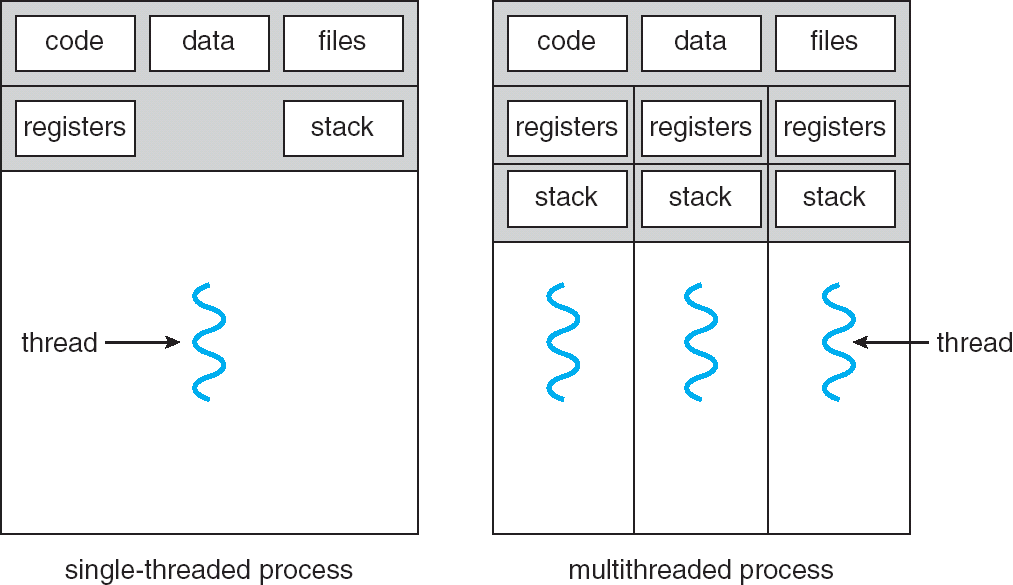
\includegraphics{pics/silberschatz7e-4-3-threads}}
\caption{Silberschatz, Gavin, Gagne: {\em Operating Systems Concepts}}
\end{figure}
\end{frame}

%---------------------------------------------------------------------- SLIDE -
\begin{frame}\frametitle{Предимства от използването на нишки}
\begin{itemize}
\item Използването на нишки води до икономия на ресурси на компютърната система
-- олекотени процеси.
\item Създаването на нишка и унищожаването на нишка изисква по-малко време.
\item Превключването на контекста между нишки става по-бързо.
\item Нишките, които са част от един и същ процес, си поделят адресното
пространство и файловете, и поради това те могат да комуникират без обръщане към
ядрото.
\item Подобрява се използването на многопроцесорните архитектури.
\end{itemize}
\end{frame}

%---------------------------------------------------------------------- SLIDE -
\begin{frame}\frametitle{Нишки}
\begin{itemize}
\item Спирането на процеса води до спиране на всички нишки на процеса, тъй като
всички нишки на процеса си поделят адресното пространство.
\item Унищожаването на процеса води до унищожаването на всички нишки на процеса.
\item Състояния на нишките:
\begin{itemize}
  \item Нова -- размножаване на нишката.
  \item Блокирана.
  \item Изпълнява се.
  \item Унищожена -- освобождава се контекста на нишката и стека.
\end{itemize}
\end{itemize}
\end{frame}

%-------------------------------------------------------------------- SECTION -
\section{Нишки в потребителското пространство}

%---------------------------------------------------------------------- SLIDE -
\begin{frame}\frametitle{Нишки в потребителското пространство}
\begin{itemize}
\item Нишките в потребителския процес съответстват на единствена нишка в ядрото.
\item Управлението на нишките се извършва от библиотека, която  изцяло работи в
потребителското пространство.
\item Ядрото по никакъв начин не знае и не се интересува от съществуването на
нишките.
\item Има редица примери за библиотеки, които поддържат нишки в потребителското
пространство:
\begin{itemize}
  \item Solaris Green Threads.
  \item GNU Portable Threads.
  \item WIN32 Threads.
\end{itemize}
\end{itemize}
\end{frame}

%---------------------------------------------------------------------- SLIDE -
\begin{frame}\frametitle{Нишки в потребителското пространство}
\begin{figure}[h]
\center
\scalebox{0.9}{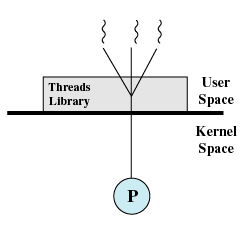
\includegraphics{pics/stallings5e-4-18-user-level-threads}}
\caption{Stallings: {\em Operating Systems: Internals and Design Principles}}
\end{figure}
\end{frame}

%---------------------------------------------------------------------- SLIDE -
\begin{frame}\frametitle{Нишки в потребителското пространство}
\begin{figure}[h]
\center
\scalebox{0.43}{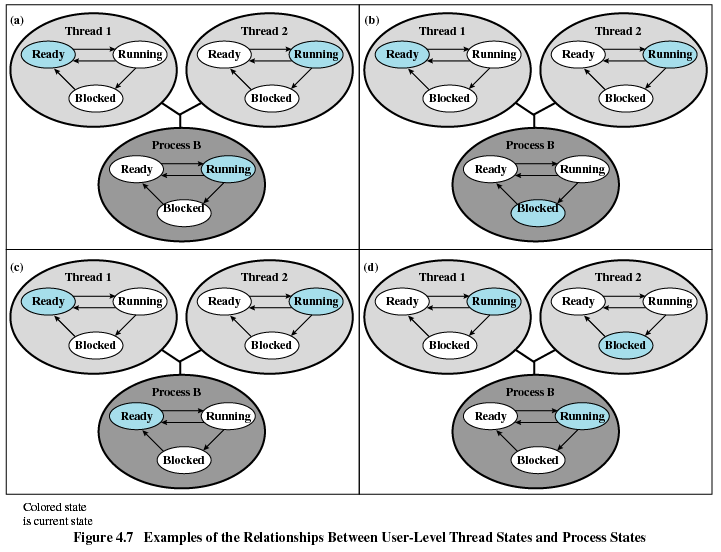
\includegraphics{pics/stallings5e-4-7-user-level-threads-and-process-state}}
\caption{Stallings: {\em Operating Systems: Internals and Design Principles}}
\end{figure}
\end{frame}


%-------------------------------------------------------------------- SECTION -
\section{Нишки в пространството на ядрото}

%---------------------------------------------------------------------- SLIDE -
\begin{frame}\frametitle{Нишки в пространството на ядрото}
\begin{itemize}
\item Всяка нишка в потребителското пространство съответстват на отделна нишка в
ядрото.
\item Изискват поддръжка в ядрото.
\item Ядрото поддържа информация за контекста на процесите и на нишките.
\item Планирането на работата на процесора е на ниво нишки.
\item Примери:
\begin{itemize}
  \item Solaris.
  \item Linux.
  \item Windows XP/2000.
  \item Tru64 UNIX.
  \item Mac OS X.
\end{itemize}
\end{itemize}
\end{frame}


%---------------------------------------------------------------------- SLIDE -
\begin{frame}\frametitle{Нишки в пространството на ядрото}
\begin{figure}[h]
\center
\scalebox{0.75}{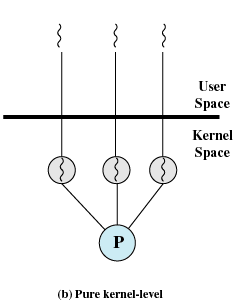
\includegraphics{pics/stallings5e-4-21-pure-kernel-level}}
\caption{Stallings: {\em Operating Systems: Internals and Design Principles}}
\end{figure}
\end{frame}


%-------------------------------------------------------------------- SECTION -
\section{Комбиниран подход}

%---------------------------------------------------------------------- SLIDE -
\begin{frame}\frametitle{Комбиниран подход}
\begin{itemize}
\item Позволява много потребителски нишки да съответстват на много нишки от
пространството на ядрото.
\item Операционната система създава достатъчен брой нишки на ядрото.
\item Планирането и синхронизацията на нишките става в рамките на
потребителското пространство.
\end{itemize}
\end{frame}

%---------------------------------------------------------------------- SLIDE -
\begin{frame}\frametitle{Комбиниран подход}
\begin{figure}[h]
\center
\scalebox{0.75}{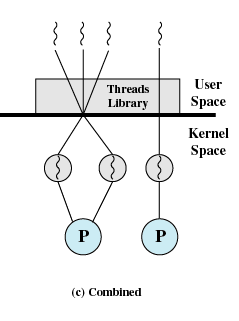
\includegraphics{pics/stallings5e-4-24-combined-threads}}
\caption{Stallings: {\em Operating Systems: Internals and Design Principles}}
\end{figure}
\end{frame}


%-------------------------------------------------------------------- SECTION -
\section{Нишки в Java}

%---------------------------------------------------------------------- SLIDE -
\begin{frame}\frametitle{Нишки в Java}
\begin{itemize}
\item Нишките в Java се управляват от JVM.
\item Има два начина да се реализират нишки в Java:
чрез наследяване на класа \lstinline{Thread} или чрез имплементация на
интерфейса \lstinline{Runnable}.
\end{itemize}
\begin{figure}[h]
\center
\scalebox{0.4}{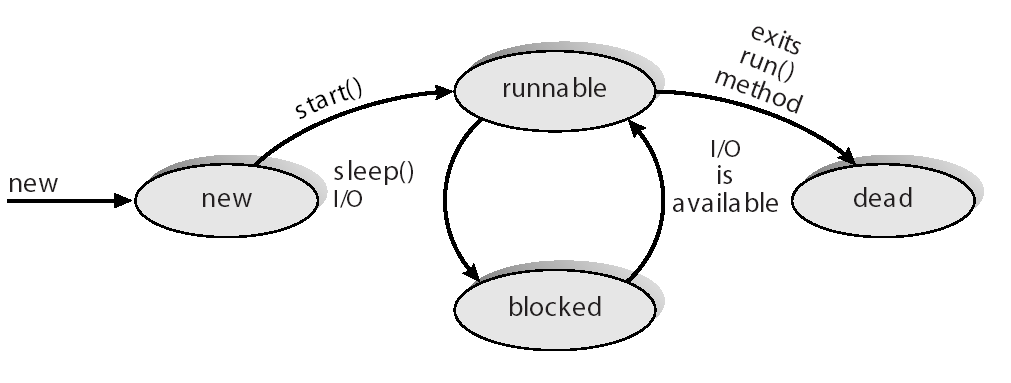
\includegraphics{pics/silberschatz7e-4-27-java-threads}}
\caption{Silberschatz, Gavin, Gagne: {\em Operating Systems Concepts}}
\end{figure}
\end{frame}

%-------------------------------------------------------------------- SECTION -
\section{Pthreads}

%---------------------------------------------------------------------- SLIDE -
\begin{frame}\frametitle{Pthreads}
\begin{itemize}
\item POSIX -- стандарт IEEE 1003.1c.
\item Дефинира стандартно API за създаване на нишки и синхронизация.
\item POSIX специфицира поведението на библиотеката.
\item Реализацията е въпрос разработка.
\item POSIX Pthreads е стандартна за UNIX операционните системи -- Solars,
Linux, Mac OS X.
\item \url{http://www.llnl.gov/computing/tutorials/pthreads/}
\end{itemize}
\end{frame}

%---------------------------------------------------------------------- SLIDE -
\begin{frame}[containsverbatim]
\frametitle{Създаване на нишки}
\begin{itemize}
\item Първоначално главната функция \lstinline{main()} разполага с единствена
нишка -- нишката на процеса. Всички останали нишки трябва изрично да бъдат
създадени.
\item Функцията \lstinline{pthread_create()} се използва за създаване на нова
нишка. Тази функция може да се вика произволен брой пъти от всяка точка на
програмата.
\item Максималният брой нишки, които могат да бъдат стартирани от един процес
зависи от имплементацията на библиотеката.
\item Веднъж създадени, нишките са равнопоставени, и могат да създавата други
нишки. Няма йерархия или зависимост между нишките.
\end{itemize}
\end{frame}

%---------------------------------------------------------------------- SLIDE -
\begin{frame}[containsverbatim]
\frametitle{Създаване на нишки}
\begin{figure}[h]
\center
\scalebox{0.4}{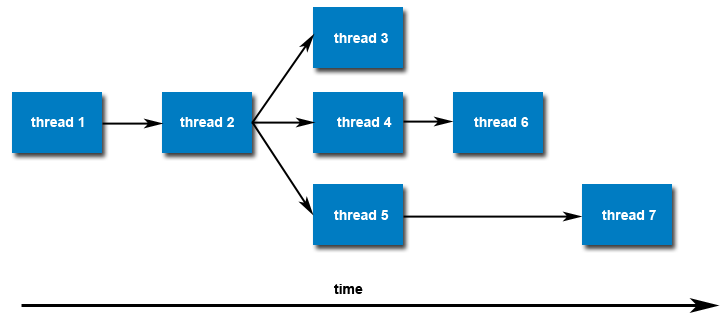
\includegraphics{pics/peerThreads}}
\caption{\url{http://www.llnl.gov/computing/tutorials/pthreads/}}
\end{figure}
\end{frame}

%---------------------------------------------------------------------- SLIDE -
\begin{frame}[containsverbatim]
\frametitle{Създаване на нишки}
\begin{lstlisting}
int pthread_create(pthread_t *thread,
    const pthread_attr_t *attr,
    void *(*start_routine)(void*), 
	void *arg);
\end{lstlisting}
Аргументите на \lstinline{pthread_create()} са:
\begin{itemize}
  \item \lstinline{thread} -- уникален идентификатор на създадената нишка.
  \item \lstinline{attr} -- специфицира атрибутите на нишката. 
  \item \lstinline{start_routine} -- функция, която се изпълнява от нишката при
  нейното стартиране.
  \item \lstinline{arg} -- аргумент, който се предава на функцията \lstinline{start_routine}.
\end{itemize}
\end{frame}

%---------------------------------------------------------------------- SLIDE -
\begin{frame}[containsverbatim]
\frametitle{Спиране на нишки}
\begin{itemize}
\item Има няколко начина, по които една Pthread нишка може да бъде унищожена:
\begin{itemize}
  \item Функцията, която се изпълнява от нишката завършва нормално работата си и
  извиква \lstinline{return}.
  \item Функцията, която се изпълнява от нишката извиква библиотечната функция
  \lstinline{pthread_exit()}.
  \item Нишката може да бъде спряна от друга нишка като се използва
  библиотечната функция \lstinline{pthread_cancel()}.
  \item Когато процеса, в който живее нишката, бъде унищожен, се унищожавт и
  всички негови нишки.
\end{itemize}
\end{itemize}
\end{frame}

%---------------------------------------------------------------------- SLIDE -
\begin{frame}[containsverbatim]
\frametitle{Спиране на нишки: \lstinline{pthread_exit()}}
\begin{lstlisting}[numbers=none]
void pthread_exit(void *value_ptr);
\end{lstlisting}
\begin{itemize}
\item Функцията \lstinline{pthread_exit()} се използва за изрично спиране на
нишка. Типично \lstinline{pthread_exit()} се извиква след като нишката е
завършила своята работа и повече не е необходима.
\item Ако главната функция \lstinline{main()} завърши работа преди нишките,
които е създала, то всички нишки също ще завършат работа. Когато обаче главната
функция \lstinline{main()} изплозва \lstinline{pthread_exit()} за завършване на
работа, останалите нишки могат да продължат да работят.
\item Функцията \lstinline{pthread_exit()} не затваря файловете, които са
отворени в рамките на нишката.
\end{itemize}
\end{frame}

%---------------------------------------------------------------------- SLIDE -
\begin{frame}[containsverbatim]
\frametitle{Пример: \lstinline{pthread}}
\lstinputlisting[lastline=11]{code/pthread01.cc}
\end{frame}


%---------------------------------------------------------------------- SLIDE -
\begin{frame}[containsverbatim]
\frametitle{Пример: \lstinline{pthread}}
\lstinputlisting[firstline=13,lastline=110]{code/pthread01.cc}
\end{frame}

%---------------------------------------------------------------------- SLIDE -
\begin{frame}[containsverbatim]
\frametitle{Пример: \lstinline{pthread}}
\begin{verbatim}
In main: creating thread 1
In main: creating thread 2
In main: creating thread 3
Hello World! It's me, thread #0!
Hello World! It's me, thread #1!
Hello World! It's me, thread #2!
In main: creating thread 4
MAIN going to exit...
Hello World! It's me, thread #3!
Hello World! It's me, thread #4!
\end{verbatim}
\end{frame}

%---------------------------------------------------------------------- SLIDE -
\begin{frame}[containsverbatim]
\frametitle{Присъединяване на нишки}
\begin{lstlisting}[numbers=none]
int pthread_join(pthread_t thread, void **value_ptr);
\end{lstlisting}
\begin{itemize}
\item Присъединяването  е начин за синхронизиране между нишки. В библиотеката
\lstinline{pthread} за присъединяване се използва функцията
\lstinline{pthread_join}. 
\item Функцията \lstinline{pthread_join()} блокира нишката, която я извиква,
докато нишката с даден идентификатор не завърши работа.
\item Всяка нишка може да бъде присъединена само веднъж. Опитът една нишка да
бъде присъединена няколко пъти е логическа грешка.
\end{itemize}
\end{frame}

%---------------------------------------------------------------------- SLIDE -
\begin{frame}[containsverbatim]
\frametitle{Присъединяване на нишки}
\begin{figure}[h]
\center
\scalebox{0.4}{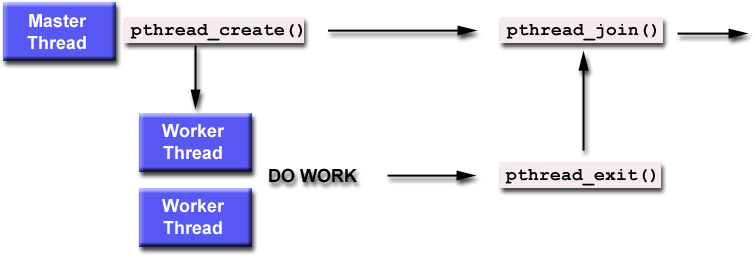
\includegraphics{pics/joiningThreads}}
\caption{\url{http://www.llnl.gov/computing/tutorials/pthreads/}}
\end{figure}
\end{frame}

%---------------------------------------------------------------------- SLIDE -
\begin{frame}[containsverbatim]
\frametitle{Пример: \lstinline{pthread}}
\lstinputlisting[lastline=14]{code/pthread02.cc}
\end{frame}


%---------------------------------------------------------------------- SLIDE -
\begin{frame}[containsverbatim]
\frametitle{Пример: \lstinline{pthread}}
\lstinputlisting[firstline=16,lastline=27]{code/pthread02.cc}
\end{frame}

%---------------------------------------------------------------------- SLIDE -
\begin{frame}[containsverbatim]
\frametitle{Пример: \lstinline{pthread}}
\lstinputlisting[firstline=29,lastline=320]{code/pthread02.cc}
\end{frame}

%---------------------------------------------------------------------- SLIDE -
\begin{frame}[containsverbatim]
\frametitle{Пример: \lstinline{pthread_join()}}
\begin{verbatim}
Creating thread 0
Creating thread 1
Creating thread 2
result = 1.073687e+15
result = 1.073788e+15
Join thread 0 status= 0
Join thread 1 status= 0
result = 1.073502e+15
Join thread 2 status= 0
\end{verbatim}
\end{frame}

\end{document}
